\documentclass[twocolumn]{ctexart}
\usepackage{fancyhdr}
\pagestyle{empty}
\usepackage{algorithmic}
\renewcommand{\algorithmicrequire}{\textbf{Input:}}
\renewcommand{\algorithmicensure}{\textbf{Output:}}
\usepackage{amssymb}
\usepackage{amsmath}
\usepackage{graphicx}
\usepackage{geometry}
\geometry{
  margin=0cm,
  left=1cm,
  right=1cm,
  headheight=0cm,
  headsep=0cm,
  top=1cm,
  bottom=1cm,
}
\setlength\parindent{0cm}
\renewcommand{\emph}[1]{\textbf{\underline{#1}}}
\begin{document}
\zihao{-6}
\begin{algorithm}
  \caption{\fbox{KNN}}%
  \label{al:knn}
  \begin{algorithmic}
    \REQUIRE$k, X = \{x_1, x_2, \ldots, x_N\}, Y = {c_1, c_2, \ldots, c_k}, x$
    \ENSURE$y$
    \STATE$N_k(x) = \arg\mathrm{sort}_{x_i}(d(x_i - x))[0:k - 1]$
    \STATE$y = \arg\max_{c_j}\sum_{x_i \in N_k(x)}\mathbb{I}(y_i = c_j)$
  \end{algorithmic}
\end{algorithm}
\begin{algorithm}
  \caption{\fbox{K Means}}%
  \label{al:k_means}
  \begin{algorithmic}
    \REQUIRE$k, X = \{x_1, x_2, \ldots, x_N\}$
    \ENSURE$q(x_i) \in \{1, \ldots, k\}$
    \FOR{$i \in \{1, \ldots, k\}$}{%
      \STATE$c_i = \mathrm{random}(X)$
    }\ENDFOR%
    \REPEAT{
      \FOR{$i \in \{1, 2, \ldots, N\}$}{%
        \STATE$q(x_i) = \arg\min_j|x_i - c_j|$
      }\ENDFOR%
      \FOR{$j \in \{1, 2, \ldots, k\}$}{%
        \STATE$c_j = \mathrm{mean}\{x_i|q(x_i) = j\}$
      }\ENDFOR%
    }\UNTIL$c_j \approx \mathrm{const}, \forall j \in \{1, 2, \ldots, k\}$
  \end{algorithmic}
\end{algorithm}
\begin{algorithm}
  \caption{\fbox{GMM}}%
  \label{al:gmm}
  \begin{algorithmic}
    \REQUIRE$k, X = \{x_1, x_2, \ldots, x_N\}$
    \ENSURE$\theta_i = [\mu_i, \sigma_i, w_i], i \in \{1, \ldots, k\}$
    \FOR{$i \in \{1, \ldots, k\}$}{%
      \STATE$\mu_i = \mathrm{random}(X)$
      \STATE$\sigma_i = \mathrm{random}()$
      \STATE$w_i = \mathrm{random}(0, 1)$
    }\ENDFOR%
    \REPEAT{
      \FOR{$i \in \{1, 2, \ldots, N\}, j \in \{1, 2, \ldots, k\}$}{%
        \STATE$\gamma_{ij} = \frac{w_j\mathcal{N}(x_i|\mathbf{\theta}_j)}
        {\sum_{j = 1}^k w_j\mathcal{N}(x_i|\theta_j)}$
      }\ENDFOR%
      \FOR{$j \in \{1, 2, \ldots, k\}$}{%
        \STATE$\mu_j = \frac{\sum_{i = 1}^N \gamma_{ij} x_i}{\sum_{i = 1}^N
        \gamma_{ij}}$
      }\ENDFOR%
      \FOR{$j \in \{1, 2, \ldots, k\}$}{%
        \STATE$\sigma_j = \frac{\sum_{i = 1}^N \gamma_{ij} {(x_i - \mu_j)}^2}
        {\sum_{i = 1}^N \gamma_{ij}}$
      }\ENDFOR%
      \FOR{$j \in \{1, 2, \ldots, k\}$}{%
        \STATE$w_j = \frac{1}{N}\sum_{i = 1}^N \gamma_{ij}$
      }\ENDFOR%
    }\UNTIL$\mathbf{\theta}_j \approx \mathrm{const}, \forall j \in \{1, 2, \ldots, k\}$
  \end{algorithmic}
\end{algorithm}
\begin{algorithm}
  \caption{\fbox{EM}}%
  \label{al:em}
  \begin{algorithmic}
    \REQUIRE$Y, Z, \mathbb{P}(Y, Z|\theta), \mathbb{P}(Z|Y, \theta)$
    \ENSURE$\theta$
    \STATE$\theta^{(0)} = \mathrm{random}()$
    \REPEAT{
      \STATE$Q(\theta, \theta^{(i)}) = \mathbb{E}_Z(\log\mathbb{P}(Y, Z|\theta)|Y, \theta^{(i)})$
      \STATE$\theta^{(i + 1)} = \arg\max_\theta Q(\theta, \theta^{(i)})$
    }\UNTIL$\theta^{(i + 1)} \approx \theta^{(i)}$
  \end{algorithmic}
\end{algorithm}
\begin{algorithm}
  \caption{\fbox{Ada Boost}}%
  \label{al:adaboost}
  \begin{algorithmic}
    \REQUIRE$X = \{x_1, x_2, \ldots, x_N\}, Y = \{y_1, y_2, \ldots, y_N\}, y_i
    \in {1, -1}, \mathscr{A}_D(X, Y): (X, Y) \rightarrow
    (G(x): X \rightarrow {-1, 1})$
    \ENSURE$G(x)$
    \FOR{$i = 1, 2, \ldots, N$}{%
      \STATE$w_{1i} = \frac1N$
    }\ENDFOR%
    \STATE$D_1 = (w_{11}, w_{12}, \ldots, w_{1N})$
    \FOR{$m = 1, 2, \ldots, M$}{%
      \STATE$G_m = \mathscr{A}_D (X, Y)$
      \STATE$e_m = \mathbb{P}(G_m(x_i) \neq y_i) = \sum_{i = 1}^N w_{mi}
      \mathbb{I}(G_m(x_i) \neq y_i)$
      \STATE$\alpha_m = \frac12\log\frac{1 - e_m}{e_m}$
      \STATE$D_{m + 1} = (w_{m + 1, 1}, w_{m + 1, 2}, \ldots, w_{m + 1, N})$
      \STATE$w_{m + 1, i} = \frac{w_{mi}\exp(-\alpha_m y_i G_m(x_i))}
      {\sum_{i = 1}^N w_{mi}\exp(-\alpha_m y_i G_m(x_i))}$
    }\ENDFOR%
    \STATE$f(x) = \sum_{m = 1}^M \alpha_m G_m(x)$
    \STATE$G(x) = \mathrm{sgn}f(x)$
  \end{algorithmic}
\end{algorithm}
\begin{algorithm}
  \caption{\fbox{Forward}}%
  \label{al:forward}
  \begin{algorithmic}
    \REQUIRE$X = \{x_1, x_2, \ldots, x_N\}, Y = \{y_1, y_2, \ldots, y_N\}$
    \ENSURE$f(x)$
    \STATE$f_0(x) = 0$
    \FOR{$m = 1, 2, \ldots, M$}{%
      \STATE$(\beta_m, \gamma_m) = \arg\min_{\beta, \gamma}\sum_{i = 1}^N L(y_i,
      f_{m - 1}(x_i) + \beta b(x_i|\gamma))$
    }\ENDFOR%
    \STATE$f_m(x) = f_{m - 1}(x) + \beta_m b(x|\gamma_m)$
    \STATE$f_m(x) = \sum_{m = 1}^M \beta_m b_m(x|\gamma_m)$
  \end{algorithmic}
\end{algorithm}
\begin{algorithm}
  \caption{\fbox{Bagging}}%
  \label{al:baggin}
  \begin{algorithmic}
    \REQUIRE$X = \{x_1, x_2, \ldots, x_N\}, Y = \{y_1, y_2, \ldots, y_N\},
    \mathscr{A}, T$
    \ENSURE$f(x)$
    \FOR{$t = 1, 2, \ldots, T$}{%
      \STATE{自助采样得到$D_\mathrm{bs}$}
      \STATE$h_t = \mathscr{A}(D_\mathrm{bs})$
    }\ENDFOR%
    \STATE$f(x) = \arg\max_{y \in Y}\sum_{t = 1}^T \mathbb(h_t(x) = y)$
  \end{algorithmic}
\end{algorithm}
\begin{algorithm}
  \caption{\fbox{Transductive Classification}}%
  \label{al:trans}
  \begin{algorithmic}
    \REQUIRE$X = \{x_1, x_2, \ldots, x_N\}, Y = \{y_1, y_2, \ldots, y_N\},
    x\prime_1, x\prime_2, \ldots, x\prime_M$
    \ENSURE$\hat{y}_j$
    \STATE{Construct a graph of $x_i, x\prime_j$ which edge's $w_{ij} =
    \frac{1}{d(x_i, x_j)}$}
    \FOR{$i = 1, 2, \ldots, N$}{%
      \STATE$p_i^{(0)} = \mathrm{onehot}(M, i)$
    }\ENDFOR%
    \REPEAT{%
      \FOR{$j \in {1, 2, \ldots, M}$}{%
        \STATE$p_j^{(t + 1)} = 0$
      }\ENDFOR%
      \FOR{$i \in {1, 2, \ldots, M + N}$}{%
        \IF{$w_{ij} \neq 0$}{%
          \STATE$p_i^{(t + 1)} = p_i^{(t)} +
          \frac{w_{ij}}{\sum_{k = 1}^M w_{ik}}p_i^{(t)}$
        }\ENDIF%
      }\ENDFOR%
      \FOR{$j \in {1, 2, \ldots, M}$}{%
        \STATE$p_j^{(t + 1)} = \frac{p_j^{(t + 1)}}{\sum_{k = 1}^M
        p_k^{(t + 1)}}$
      }\ENDFOR%
    }\UNTIL$p_j^{(t + 1)} \approx p_j^{(t)}$
    \FOR{$j \in {1, 2, \ldots, M}$}{%
      \STATE$\hat{y}_j = \arg\max{p_j^{(t + 1)}}$
    }
  \end{algorithmic}
\end{algorithm}
\begin{algorithm}
  \caption{\fbox{Page Rank}}%
  \label{al:page_rank}
  \begin{algorithmic}
    \REQUIRE{A graph of webpages and hyperlinks}
    \ENSURE{Relative importance values of all webpages $r_j$}
    \FOR{$i = 1, 2, \ldots, N$}{%
      \STATE$r_i^{(0)} = \mathrm{random}()$
    }\ENDFOR%
    \REPEAT{%
      \FOR{$j \in {1, 2, \ldots, M}$}{%
        \STATE$r_j^{(t + 1)} = 0$
      }\ENDFOR%
      \FOR{$j \in {1, 2, \ldots, M}$}{%
        \IF{$w_{ij} \neq 0$}{%
          \STATE$r_i^{(t + 1)} = r_i^{(t)} +
          \frac{w_{ij}}{\sum_{k = 1}^M w_{ik}}r_i^{(t)}$
        }\ENDIF%
      }\ENDFOR%
      \FOR{$j \in {1, 2, \ldots, M}$}{%
        \STATE$r_j^{(t + 1)} = \beta r_j^{(t)} + \frac{1 - \beta}{N}$
      }\ENDFOR%
    }\UNTIL$r_j^{(t + 1)} \approx r_j^{(t)}$
  \end{algorithmic}
\end{algorithm}
\begin{algorithm}
  \caption{\fbox{ID3}}%
  \label{al:id3}
  \begin{algorithmic}
    \REQUIRE$D, A, \epsilon$
    \ENSURE$T$
    \IF{$D$中所有实例都属于同一类$C_k$}{%
      \STATE{构建单结点树$T$,并将类$C_k$作为该结点的类标记}
      \RETURN$T$
    }\ENDIF%
    \IF{$A = \emptyset$}{%
      \STATE{构建单结点树$T$,并将$D$中实例数最大的类$C_k$作为该结点的类标记}
      \RETURN$T$
    }\ENDIF%
    \STATE$A_g = \arg\max_{a \in A}G(a)$
    \IF{$G(A_g) < \epsilon$}{%
      \STATE{构建单结点树$T$,并将$D$中实例数最大的类$C_k$作为该结点的类标记}
      \RETURN$T$
    }\ENDIF%
    \FOR{$a_i \in A_g$}{%
      \STATE{依照$A_g = a_i$将$D$分割为若干非空子集$D_i$,将$D_i$中实例数最大的
      类作为标记,构建子结点}
      \FOR{第$i$个子结点}{%
        \STATE$T_i = \mathrm{ID3}(D_i, A - A_g, \epsilon)$
      }\ENDFOR%
    }\ENDFOR%
    \STATE{所有的结点和其子结点构成树$T$}
    \RETURN$T$
  \end{algorithmic}
\end{algorithm}
\begin{algorithm}
  \caption{\fbox{Cut}}%
  \label{al:cut}
  \begin{algorithmic}
    \REQUIRE$T, \alpha$
    \ENSURE$T_\alpha$
    \FOR{每个结点}{%
      \STATE{计算每个结点的经验熵}
    }\ENDFOR%
    \REPEAT{%
      \STATE{从树的叶结点往上回缩,设回缩前后的树分别为$T_0, T_1$}
      \IF{$C_\alpha(T_1) \leqslant C_\alpha(T_0)$}{%
        \STATE{剪枝}
      }\ENDIF%
    }\WHILE{不能继续剪枝}
    \RETURN$T_\alpha$
  \end{algorithmic}
\end{algorithm}
\begin{algorithm}
  \caption{\fbox{Perceptron}}%
  \label{al:perceptron}
  \begin{algorithmic}
    \REQUIRE$X = \{x_1, x_2, \ldots, x_N\}, Y = \{y_1, y_2, \ldots, y_N\}, y_i \in {1, -1}, \eta$
    \ENSURE$w, b$
    \STATE$w_0 = \mathrm{random}()$
    \STATE$b_0 = \mathrm{random}()$
    \REPEAT{%
      \STATE$(x_i, y_i) = \mathrm{random}(X, Y)$
      \IF{$y_i(\mathbf{w}^\mathsf{T}\mathsf{x}_i + b) < 0$}{%
        \STATE$w^{(t + 1)} = w^{t} + \eta y_i x_i$
        \STATE$b^{(t + 1)} = b^{t} + \eta y_i$
      }\ENDIF%
    }\UNTIL{无误分类点}
  \end{algorithmic}
\end{algorithm}

\fbox{Formulate}

$R$ is radius of data point

$y = \mathbb{I}_{\pm1}(w \cdot x + b \geqslant \Delta)$

$d_\mathrm{SVM} \leqslant \min(\mathrm{size}(x), \frac{R^2}{\Delta^2}) + 1$

$N_\mathscr{F}(x_1, x_2, \ldots, x_N) = |\{f(x_1|\alpha), f(x_2|\alpha),
\ldots, f(x_N|\alpha)|f \in \mathscr{F}\}|$

$H_\mathscr{F}(m) = \mathbb{E}_{\mathrm{size}(x) = m}\log(N_\mathscr{F}(x))$

$\hat{H}_\mathscr{F}(m) = \log(\mathbb{E}_{\mathrm{size}(x) = m}N_\mathscr{F}(x))$

$G_\mathscr{F}(m) = \log(\max_{\mathrm{size}(x) = m}N_\mathscr{F}(x))$

$G_\mathscr{F}(m) \leqslant \sum_{i = 1}^d \binom{m}{i}$

$G(D) = 1 - \sum p_i^2$

$g = H(D) - \sum\frac{|D_i|}{|D|}H(D_i)$

$gr = \frac{g}{-\sum\frac{D_i}{D}\log\frac{|D_i|}{|D|}}$

\begin{align}
  L(w) & = \sum_{i = 1}^N(y_i\log p(x_i) + (1 - y_i)\log(1 - p(x_i)))\\
       & = \sum_{i = 1}^N(y_i\log \frac{p(x_i)}{1 - p(x_i)} + \log(1 - p(x_i)))\\
       & = \sum_{i = 1}^N(y_i(w \cdots x_i) - \log(1 + \exp(w \cdot x_i)))
\end{align}
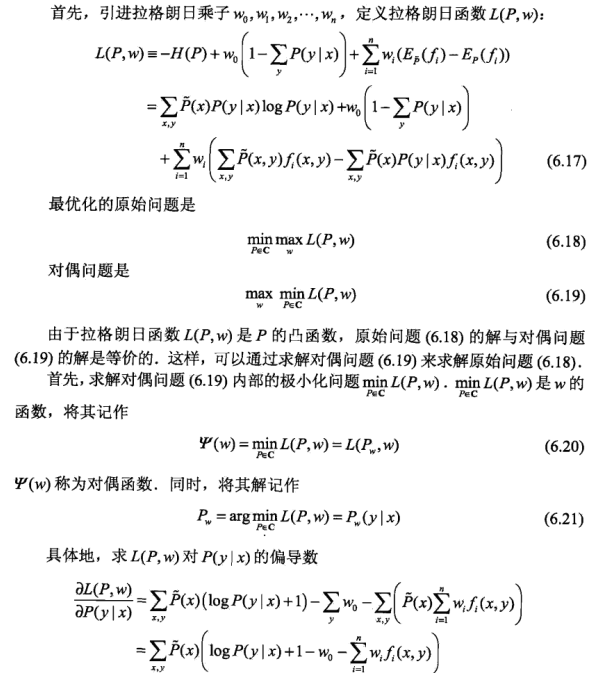
\includegraphics[
  width=\linewidth,
]{images/1.png}
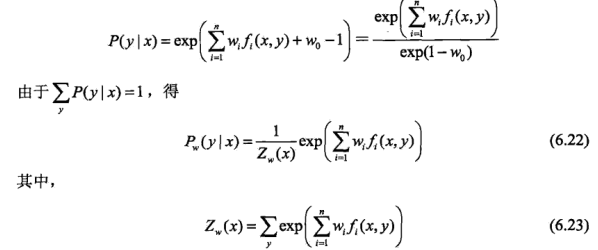
\includegraphics[
  width=\linewidth,
]{images/2.png}
\end{document}
